% !TEX encoding = UTF-8
% !TEX TS-program = pdflatex
% !TEX root = ../tesi.tex

\subsection{UC4 - Visualizzazione procedimenti}
\begin{itemize}
  \item \textbf{Identificativo}: UC4
  \item \textbf{Nome}: visualizzazione procedimenti
  \item \textbf{Descrizione grafica}:
\end{itemize}

\begin{figure}[H]
  \centering
  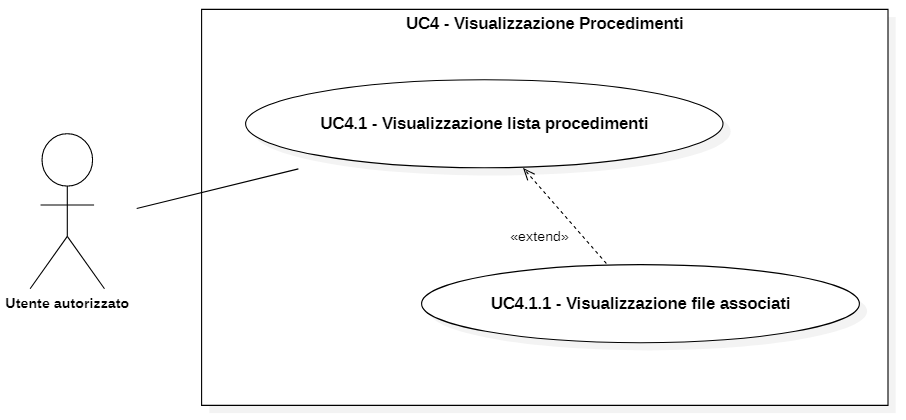
\includegraphics[width=\textwidth]{immagini/usecase/UC4.png}
  \caption{Descrizione grafica caso d'uso UC4}
\end{figure}

\begin{itemize}
  \item \textbf{Attori}
        \begin{itemize}
          \item \textit{Primari}: utente autorizzato
        \end{itemize}
  \item \textbf{Precondizione}: l'utente ha già effettuato correttamente il caricamento dati da CD.
  \item \textbf{Postcondizione}: l'utente visualizza i procedimenti relativi ai dati caricati.
  \item \textbf{Scenario principale}: l'utente da questa vista, può visualizzare la lista dei procedimenti e i file relativi ad ognuno.
  \item \textbf{Scenario principale}: l'utente può modificare i metadati di ogni procedimento. (\textbf{UC5.1})
\end{itemize}

\subsubsection{UC4.1 - Visualizzazione lista procedimenti}
\begin{itemize}
  \item \textbf{Identificativo}: UC4.1
  \item \textbf{Nome}: visualizzazione lista procedimenti
  \item \textbf{Descrizione grafica}: (approfondita in UC4)
  \item \textbf{Attori}
        \begin{itemize}
          \item \textit{Primari}: utente autorizzato
        \end{itemize}
  \item \textbf{Precondizione}: l'utente si trova sulla pagina di elenco procedimenti.
  \item \textbf{Postcondizione}: l'utente visualizza la lista dei procedimenti ognuno con i relativi file.
  \item \textbf{Scenario principale}: l'utente visualizza la lista dei procedimenti e può visualizzare la lista dei file associati.
  \item \textbf{Scenario secondario}: l'utente può visualizzare la lista dei file associati ad ogni procedimento.
\end{itemize}

\subsubsection{UC4.1.1 - Visualizzazione file associati}
\begin{itemize}
  \item \textbf{Identificativo}: UC4.1.1
  \item \textbf{Nome}: visualizzazione file associati
  \item \textbf{Descrizione grafica}: (approfondita in UC4)
  \item \textbf{Attori}
        \begin{itemize}
          \item \textit{Primari}: utente autorizzato
        \end{itemize}
  \item \textbf{Precondizione}: l'utente si trova sulla pagina di elenco procedimenti.
  \item \textbf{Postcondizione}: l'utente visualizza la lista dei fie associati ad un procedimento.
  \item \textbf{Scenario principale}: l'utente visualizza la lista dei procedimenti e con un apposito bottone può visualizzare la lista dei file associati.
\end{itemize}
\newpage